\section{\textit{Benchmarking} Automatizzato per il Confronto Prestazionale tra Librerie}

Al fine di condurre un'analisi comparativa rigorosa e sistematica delle prestazioni offerte dalle diverse librerie di visualizzazione cartografica prese in esame, è stato realizzato un progetto separato il quale implementa una specifica funzionalità di benchmarking automatizzato. Questo sistema è stato impiegato per acquisire misurazioni quantitative e ripetibili dei tempi di esecuzione e rendering, minimizzando al contempo l'intervento manuale e le potenziali distorsioni da esso derivanti. Si è posta particolare enfasi nel garantire che ogni singola prova venisse eseguita in condizioni operative il più possibile isolate e \say{pulite}, ovvero esenti da interferenze dovute a stati precedenti dell'applicazione o a risorse memorizzate nella cache.
Grazie a tali dati, è stato possibile valutare la reattività di ogni libreria considerata e presentare, in questo elaborato, un'analisi concisa e fruibile.

Il fulcro di questa architettura di test è rappresentato da un'istanza di Flask che mette a disposizione una pagina web dedicata, accessibile tramite l'endpoint applicativo \texttt{/benchmark}. 
È doveroso specificare come in queste misurazioni non è stato incluso \textit{Folium}; tale libreria si differenzia dalle altre per via del suo diverso funzionamento, infatti non è possibile effettuare un \textit{benchmark} significativo tra librerie \textit{server-side rendered} (SSR) e \textit{client-side rendered} (CSR) a causa delle differenze fondamentali nei loro modelli di \textit{rendering} e nei flussi di esecuzione. 

Nello specifico:
\begin{itemize}
      \item Server-Side Rendering (SSR): Il contenuto HTML completo viene generato sul server e inviato al client. Questo approccio consente una visualizzazione immediata del contenuto e una migliore indicizzazione da parte dei motori di ricerca.\cite{peerdh-ssr-csr-comparison}

    \item Client-Side Rendering (CSR): Il server invia una struttura HTML minima, e il browser del client utilizza JavaScript per costruire dinamicamente l'interfaccia utente. Questo può comportare un ritardo nella visualizzazione iniziale del contenuto e richiede che il browser esegua ulteriori elaborazioni.\cite{devto-csr-vs-ssr}
\end{itemize}
  

Il processo di benchmarking si articola nelle seguenti fasi operative fondamentali:

\begin{itemize}[leftmargin=*]
    \item \textbf{Caricamento Iterativo e Contestualizzato delle Mappe:}
    Per ogni libreria inclusa nel ciclo di test e per ciascuna iterazione configurata, la corrispondente pagina web dedicata alla visualizzazione della mappa (ad esempio, \texttt{/leaflet}, \texttt{/openlayers}, ecc.) viene caricata dinamicamente all'interno di un elemento HTML \texttt{<iframe>}. Quest'ultimo è integrato nella pagina di \textit{benchmark} e serve a creare un ambiente di esecuzione \textit{sandboxed} per ogni test. Questo approccio consente di caricare, inizializzare e renderizzare ogni mappa in un contesto di DOM e JavaScript relativamente isolato, riducendo le possibili interferenze tra test successivi. Sebbene l'\textit{iframe} possa essere configurato per essere invisibile durante l'esecuzione standard, la sua visibilità può essere attivata a fini diagnostici e di \textit{debug}.

    \item \textbf{Implementazione di Strategie Anti-Cache Robuste:}
    Una criticità fondamentale nei test di performance web è l'influenza della cache del browser. Per assicurare che ogni caricamento della mappa avvenga ex novo, attingendo le risorse direttamente dal server (o dalla rete, nel caso di \textit{CDN} esterne), sono state implementate due strategie anti-\textit{cache} complementari e sinergiche:
    \begin{itemize}
        \item \textit{Direttive HTTP Server-Side:} Il server applicativo Flask è stato configurato per apporre, a tutte le risposte HTTP generate, specifiche intestazioni di controllo della cache. Tra queste, le più interessanti sono \texttt{Cache-Control: no-cache, no-store, must-revalidate}, \texttt{Pragma: no-cache}, e \texttt{Expires: 0}, le quali istruiscono esplicitamente il browser a non riutilizzare versioni precedentemente memorizzate delle risorse, ma a richiederle nuovamente.
        \item \textit{Parametrizzazione Dinamica degli URL Client-Side:} In aggiunta alle direttive server-side, un meccanismo di \say{\textit{cache busting}} è applicato lato client. Ad ogni URL della pagina mappa da caricare nell'\textit{iframe} viene programmaticamente aggiunto un parametro di query univoco, tipicamente basato sul \textit{timestamp} corrente (es. \texttt{?t=xxxxxxxxxxxxx}). Questa tecnica rende ogni richiesta URL formalmente distinta dalla precedente agli occhi del browser, contribuendo significativamente a vanificare i meccanismi di \textit{caching} più aggressivi.
    \end{itemize}

    \item \textbf{Raccolta Differita e Asincrona delle Metriche di Performance:}
    La misurazione effettiva delle prestazioni è delegata a ciascuna singola pagina di visualizzazione della mappa. All'interno dello script di ogni pagina mappa (es. \texttt{leaflet.html}), vengono utilizzati meccanismi di timing ad alta precisione, come \texttt{performance.now()}, per registrare gli istanti di inizio e fine delle operazioni chiave: recupero dei dati, inizializzazione della mappa base e rendering dello strato \textit{heatmap}.
    Una volta che tutte queste operazioni sono concluse e le metriche sono state calcolate, la pagina mappa ospitata nell'\textit{iframe} emette un evento JavaScript personalizzato, denominato \texttt{benchmarkMetricsReady}, sull'oggetto \texttt{window} del proprio contesto. Il \textit{payload} associato a questo evento (\texttt{event.detail}) è un oggetto JSON contenente tutte le metriche rilevate (per esempio \texttt{dataFetchTime\_ms}, \texttt{mapInitAndHeatmapRenderTime\_ms}, \texttt{totalClientLoadTime\_ms}, \texttt{totalPoints}). La pagina genitore \texttt{/benchmark} si pone in \textit{ascolto attivo} di questo specifico evento proveniente dall'\textit{iframe}, per poter intercettare e registrare i dati di performance non appena disponibili.

    \item \textbf{Aggregazione, Formattazione e Persistenza dei Dati:}
    Le metriche raccolte per ogni singola iterazione di test vengono progressivamente accumulate in una struttura dati (un array JavaScript) nella pagina \texttt{/benchmark}. Questa struttura include non solo le misurazioni temporali, ma anche metadati contestuali quali il nome della libreria mappa testata, il numero progressivo dell'iterazione e la stringa completa dello User-Agent del browser che ha eseguito il test.
    Al completamento di tutte le iterazioni per tutte le librerie configurate, l'intero \textit{dataset} di risultati viene serializzato in formato JSON e trasmesso, tramite una richiesta HTTP di tipo POST, a un endpoint server-side dedicato: \texttt{/save\_benchmark\_data}. Questo endpoint, gestito dall'applicazione Flask, riceve i dati e provvede ad accodarli in modo persistente a un file testuale formattato come CSV (Comma-Separated Values); è possibile consultare un estratto di poche righe di tale file, disposto in Tabella \ref{tab:csv-metriche-mappe}, in cui viene mostrato come vengono organizzate le misurazioni. Il file, denominato \texttt{benchmarks.csv} e localizzato nella directory radice del progetto, funge da archivio storico di tutte le sessioni di \textit{benchmark}. La sua struttura tabellare, con colonne chiaramente definite, facilita l'analisi successiva e il confronto dei dati, permettendo l'importazione in fogli di calcolo o software statistici.
        
\end{itemize}

\begin{table}[ht]
\centering
\caption{Esempio di dati raccolti per \textit{Leaflet}} % Added descriptive caption
\label{tab:csv-metriche-mappe}
\sisetup{
  output-exponent-marker=\text{\,E\,},
  exponent-product={},
  group-digits=false
}
\begin{tabular}{
  l
  S[table-format=1.0]
  S[table-format=5.0]
  S[table-format=3.2]
  S[table-format=3.0]
}
\toprule
\textbf{Mappa} & \textbf{Iterazioni} & \textbf{Punti totali} & \textbf{Data Fetch (ms)} & \textbf{Map Init \& Render (ms)} \\
\midrule
Leaflet & 1 & 76533 & 502.75 & 580 \\
Leaflet & 2 & 76533 & 487.70 & 561 \\
Leaflet & 3 & 76533 & 480.63 & 546 \\
Leaflet & 4 & 76533 & 468.64 & 536 \\
Leaflet & 5 & 76533 & 462.73 & 539 \\
\vdots  &\vdots  &\vdots  &\vdots  &\vdots \\
Leaflet & 46 & 76533 & 455,67 & 526 \\
Leaflet & 47 & 76533 & 508,65 & 577 \\
Leaflet & 48 & 76533 & 594.60 & 658 \\
Leaflet & 49 & 76533 & 456.62 & 520 \\ 
Leaflet & 50 & 76533 & 499.65 & 568 \\
\bottomrule
\end{tabular}
\end{table}


% focus sul benchmark
\subsection{Metodologia di Rilevamento delle Metriche}

Il sistema di \textit{benchmarking} automatizzato esegue 50 iterazioni per ciascuna libreria cartografica. In ogni iterazione, vengono misurate tre metriche principali: il tempo di recupero dei dati (\textit{data fetch time}), il tempo di inizializzazione e \textit{rendering} della mappa (\textit{map initialization and heatmap render time}) e il tempo totale di caricamento (\textit{total client load time}). Il processo di misurazione inizia quando l'utente richiede la visualizzazione della mappa e termina quando la \textit{heatmap} è completamente renderizzata e interattiva. Per ogni libreria, è stato implementato un sistema di eventi personalizzato che marca con precisione i momenti chiave del ciclo di vita della mappa:

\begin{itemize}
    \item \textbf{Tempo di Recupero Dati}: Misurato dall'inizio della richiesta HTTP fino al completamento del download dei dati dei punti. Questo intervallo è calcolato utilizzando l'API Performance del browser, specificamente attraverso il \texttt{PerformanceNavigationTiming}.

    \item \textbf{Tempo di Inizializzazione e Rendering}: Calcolato dall'istante in cui i dati sono disponibili fino al completamento del rendering della heatmap. Per ogni libreria, questo evento è segnalato in modo specifico:
    \begin{itemize}
        \item \textbf{Leaflet}: Utilizza l'evento \texttt{layeradd} del plugin \texttt{Leaflet.heat} per rilevare l'aggiunta del layer heatmap alla mappa \cite{leaflet-heat}.
        \item \textbf{MapLibre GL JS}: Monitora l'evento \texttt{sourcedata} con controllo dello stato \texttt{loaded} per determinare quando i dati della sorgente sono completamente caricati \cite{maplibre-sourcedata}.
        \item \textbf{OpenLayers}: Sfrutta l'evento \texttt{postrender} del layer heatmap per identificare il completamento del rendering \cite{openlayers-heatmap}.
        \item \textbf{Deck.gl}: Utilizza il callback \texttt{onAfterRender} del componente per rilevare quando il rendering è stato completato \cite{deckgl-onafterrender}.
    \end{itemize}

    \item \textbf{Tempo Totale di Caricamento}: Rappresenta la somma del tempo di recupero dati e del tempo di inizializzazione e rendering, fornendo una metrica complessiva dell'esperienza utente.
\end{itemize}

Riassumendo, ogni iterazione di questo test viene eseguita in un \textit{iframe} isolato per evitare interferenze tra le diverse esecuzioni. Le metriche vengono raccolte lato client attraverso un evento personalizzato \texttt{benchmarkMetricsReady} che viene \textit{dispatchato} al completamento di ogni ciclo di \textit{rendering}. I dati raccolti vengono quindi aggregati e salvati in un file CSV per l'analisi successiva. Questo approccio metodico assicura che le misurazioni siano rappresentative delle reali prestazioni di ciascuna libreria in un contesto applicativo reale.


\subsection{Analisi sulla Correlazione delle Metriche}
\begin{figure}[!ht]
    \centering
    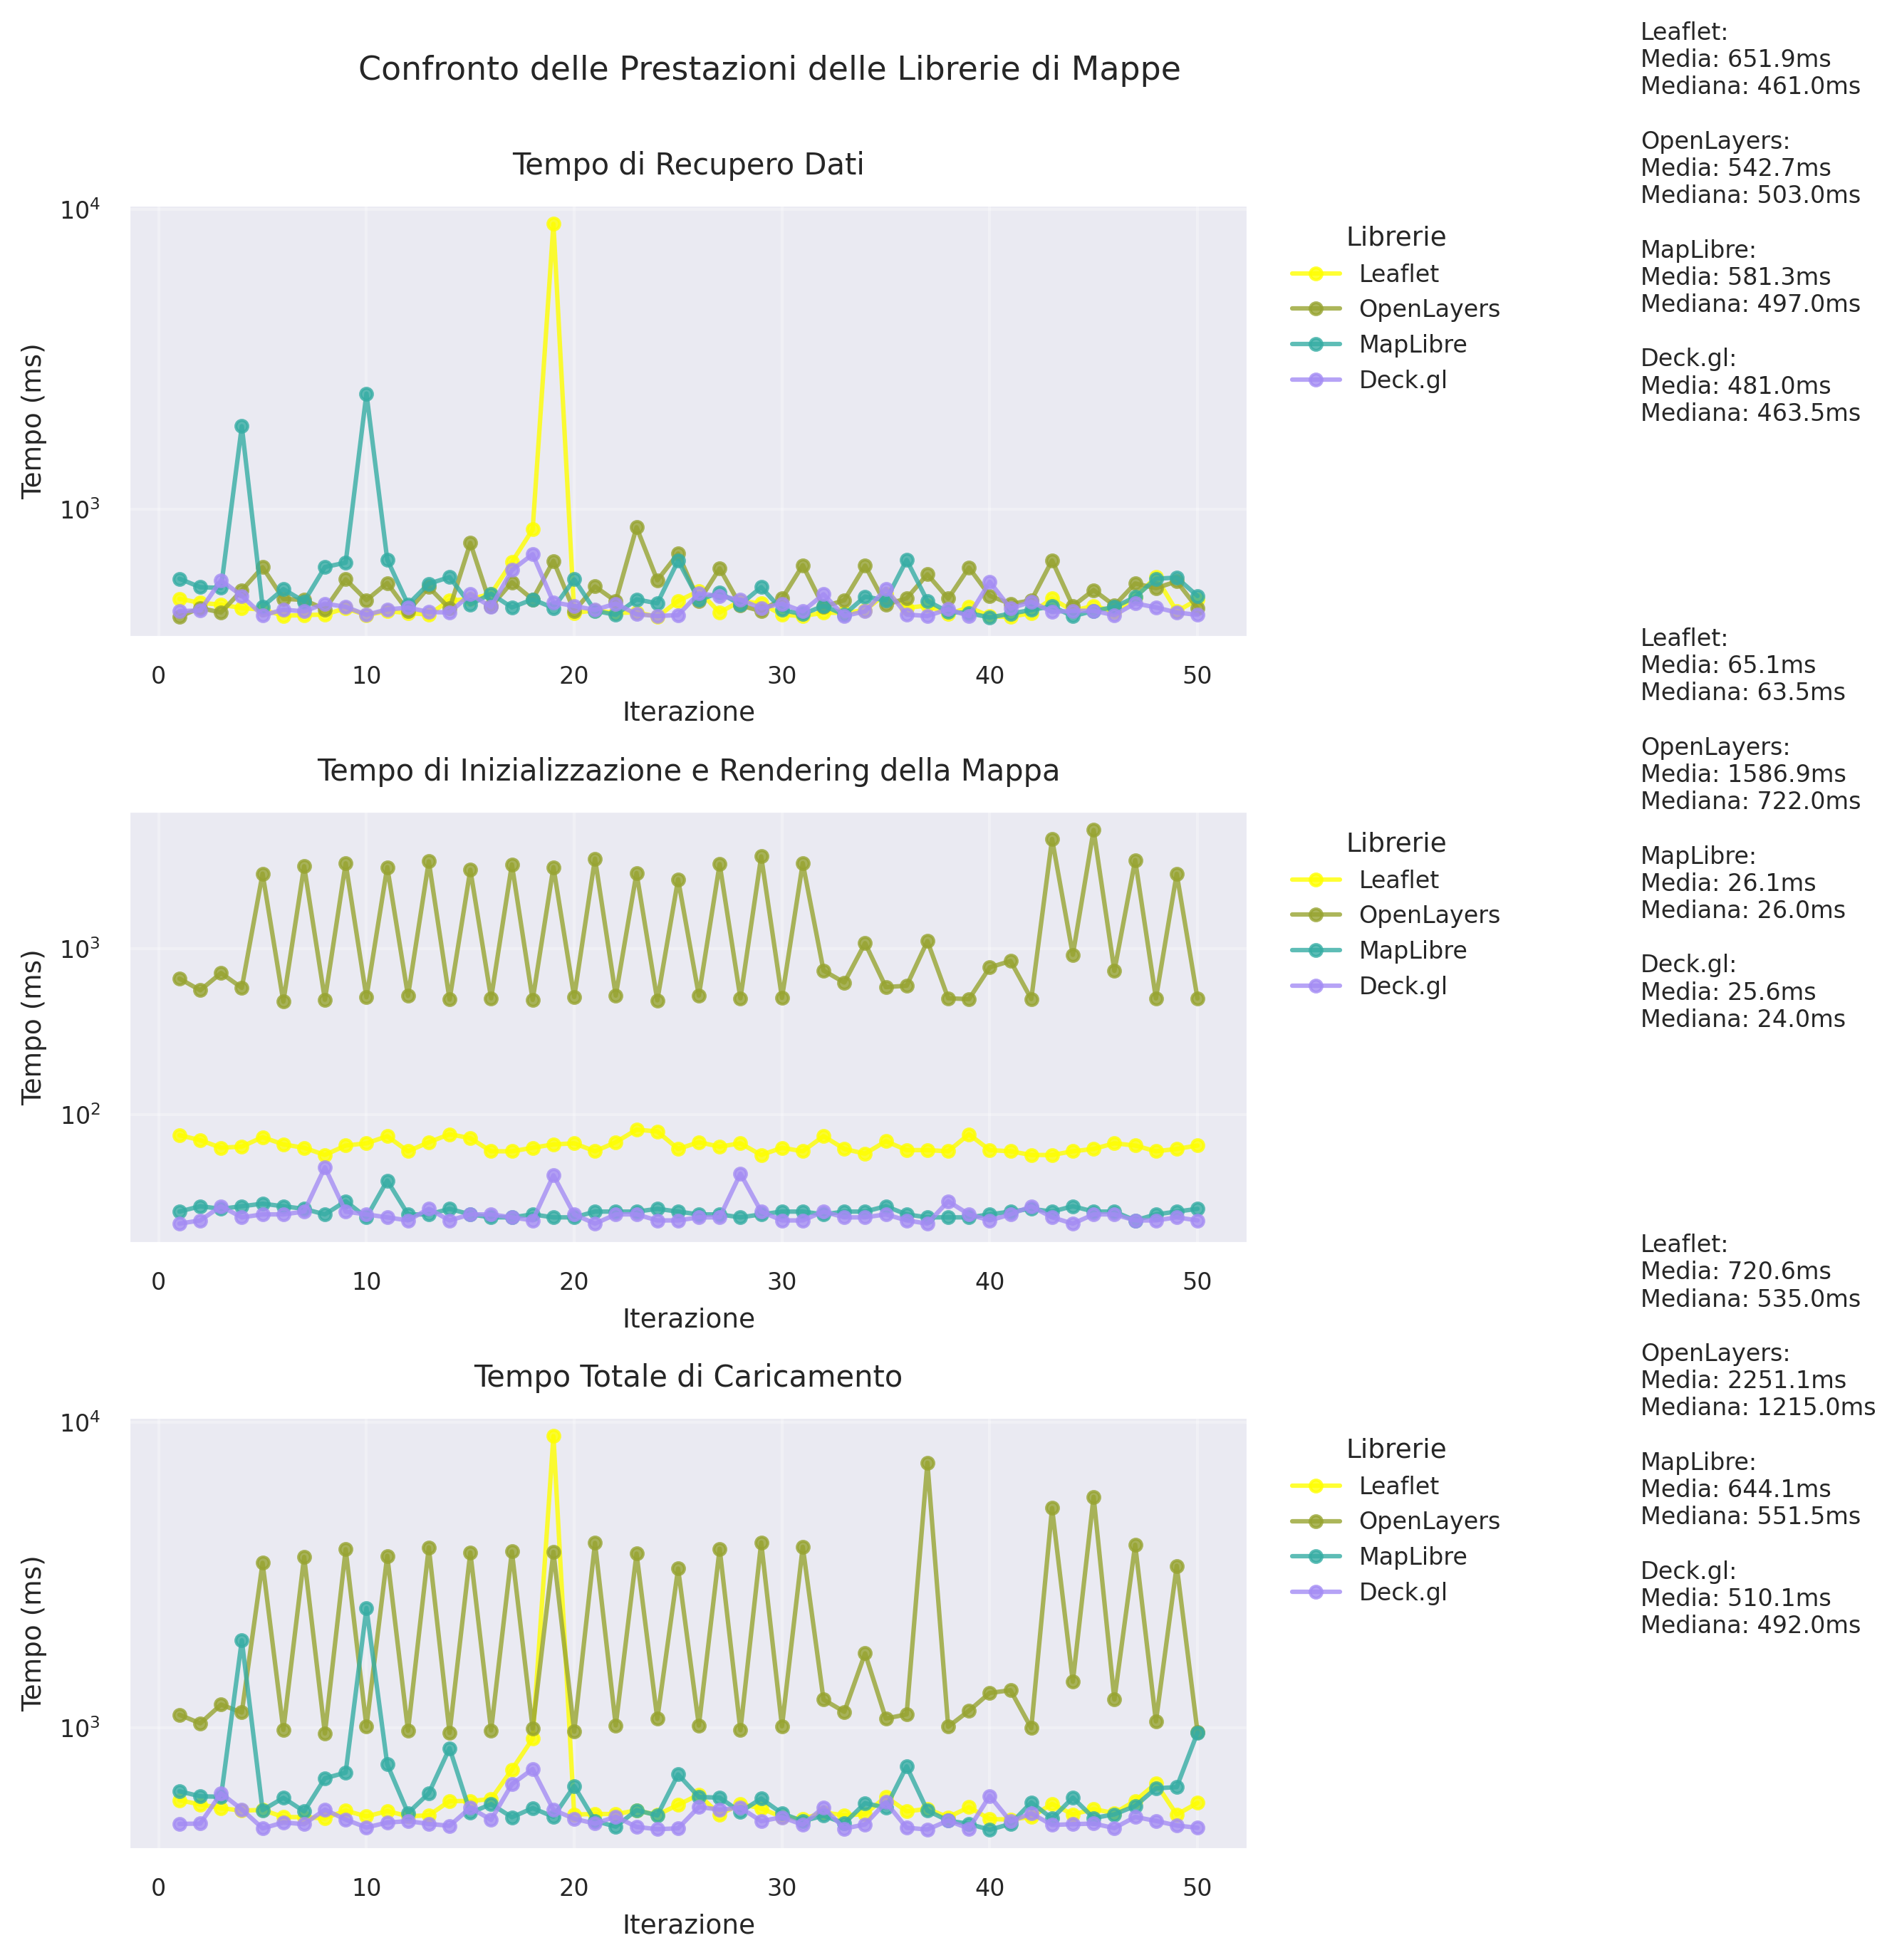
\includegraphics[width=\textwidth]{chapters/librerie-plot/data/confronto_benchmark.png}
    \captionsetup{justification=centering}
    \caption{Grafico combinato di Tempo di caricamento dati,\\ di Inizializzazione Mappa, e Rendering Heatmap}
    \label{fig:map_benchmark}
\end{figure}

\begin{figure}[!ht]
    \centering
    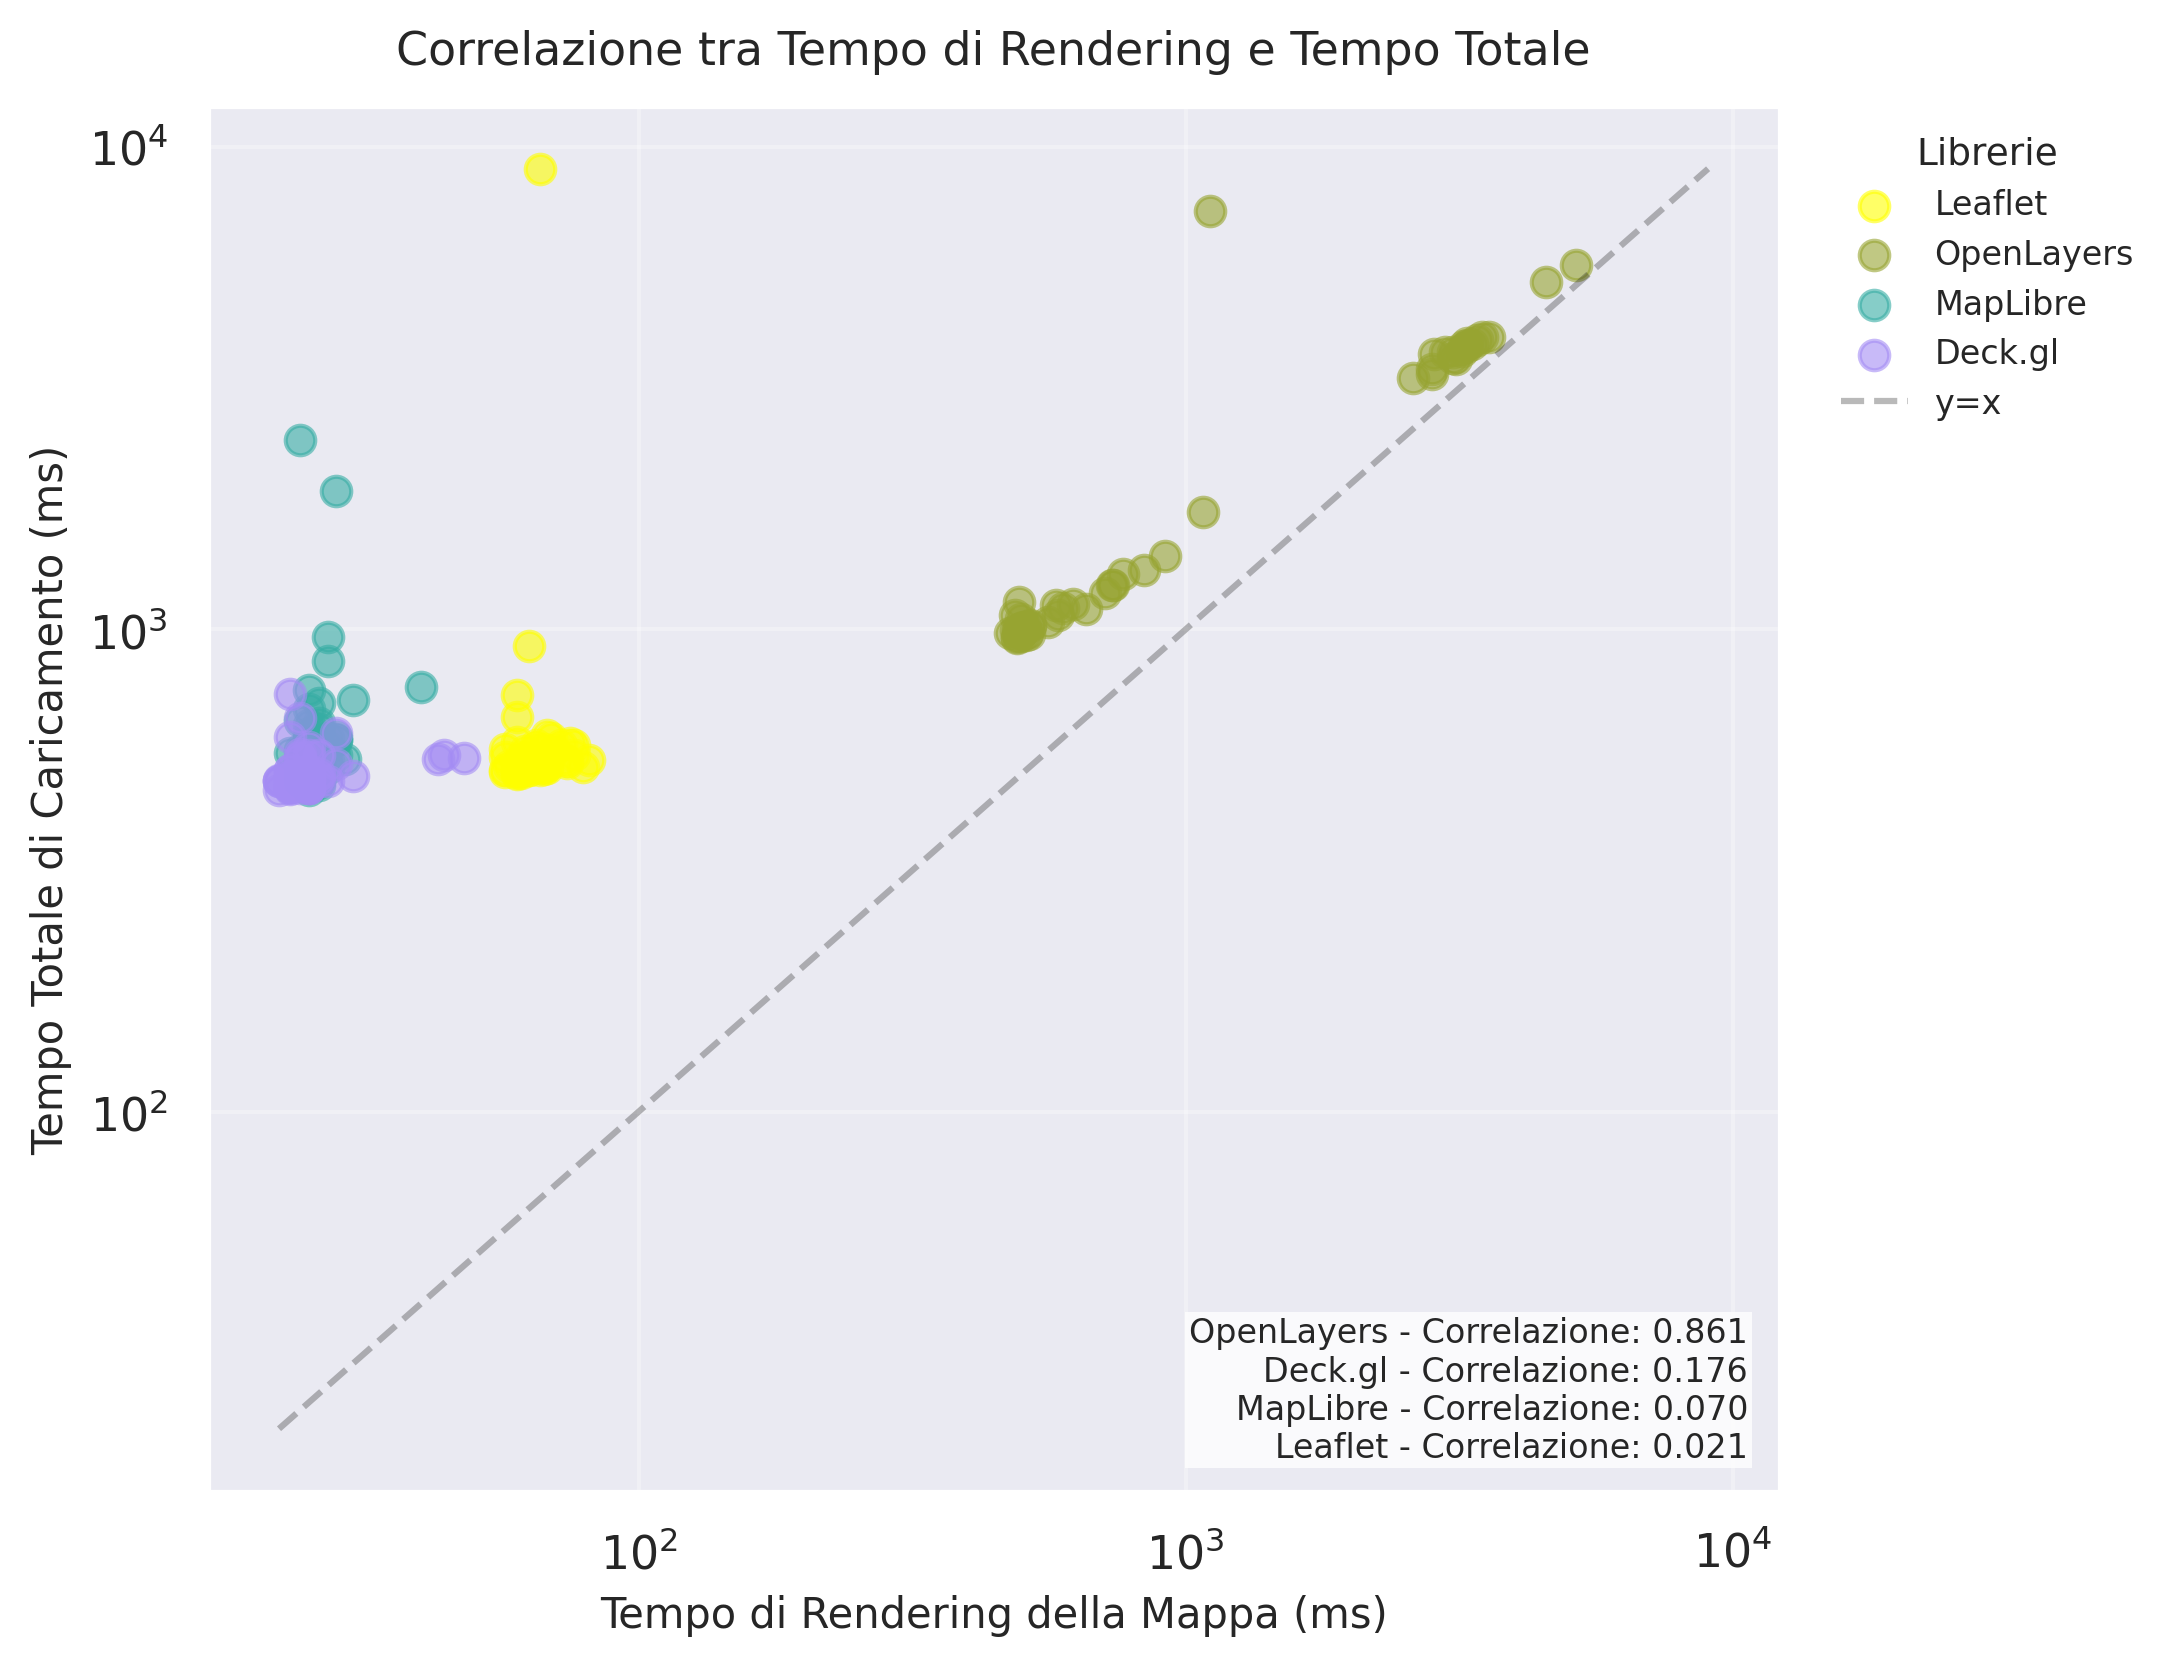
\includegraphics[width=\textwidth]{chapters/librerie-plot/data/correlazione_rendering_totale.png}
    \caption{Grafico che unisce tempo di Inizializzazione Mappa e Rendering Heatmap}
    \label{fig:map_xy_plot}
\end{figure}



% commento grafico linee
Come illustrato in Figura \ref{fig:map_benchmark}, il grafico riassume le prestazioni delle librerie poste in analisi, in relazione alle metriche chiave di caricamento. Le linee presenti nei grafici delineano l'andamento dei dati rilevati e permettono di valutare in modo visivo i punti di forza e di debolezza di ciascuna soluzione.

Nello specifico, il grafico mette a confronto i seguenti dati rilevati:
    \begin{itemize}
        \item Tempo di Recupero dei Dati Geospaziali
        \item Tempo di Inizializzazione e Rendering della Mappa
        \item Tempo totale di Caricamento
    \end{itemize}
    

L'asse \textbf{verticale} rappresenta il tempo in millisecondi impiegato, mentre l'asse \textbf{orizzontale} categorizza la sequenza di rilevazioni ottenute.

Si osserva che le librerie Deck.gl e MapBox/MapLibre eccellono particolarmente nel tempo di inizializzazione e rendering, seguite da Leaflet, registrando i valori più bassi, il che le rende una scelta ottimale per scenari in cui tale aspetto è critico. Al contrario, la libreria OpenLayers mostra prestazioni meno competitive nello stesso ambito, suggerendo aree che richiedono potenziale ottimizzazione o che la rendono meno adatta per carichi di lavoro specifici.

È interessante notare come Leaflet e Deck.gl mostrino prestazioni simili e costantemente basse per il tempo di rendering e OpenLayers presenti una variabilità maggiore per il tempo totale di caricamento. Questo potrebbe indicare fattori architetturali comuni, diverse strategie di ottimizzazione, o impatti di terze parti meno controllabili.

L'analisi di questo grafico di confronto è fondamentale per orientare la scelta della libreria più adatta alle esigenze specifiche del progetto. Essa rivela non solo le performance assolute, ma anche le loro caratteristiche relative, permettendo di identificare la soluzione che meglio si allinea ai requisiti di velocità e reattività dell'applicazione finale.

% commento grafico xy
Ora prendiamo in considerazione ciò che viene illustrato in Figura \ref{fig:map_xy_plot}. Questo  grafico di dispersione presenta la relazione tra il tempo impiegato per il \textbf{rendering della mappa} (misurato in millisecondi sull'asse delle ascisse) e il \textbf{tempo totale di caricamento lato client} (misurato in millisecondi sull'asse delle ordinate). Ogni punto sul grafico rappresenta una singola osservazione di test, e le diverse librerie cartografiche (Leaflet, OpenLayers, MapLibre, Deck.gl), ognuna differenziata da un colore diverso, permettono di distinguere visivamente i loro rispettivi comportamenti.

\begin{itemize}
    \item \textbf{Limite inferiore}
    Si osserva una disposizione dei dati ben definita, dove nessuna libreria è in grado di raggiungere tempi totali di caricamento sotto una certa soglia (indicativamente, $\sim 500$ ms). Interessante la disposizione dei \textit{datapoints} lungo l'asse delle ascisse, quindi l'asse lungo il quale sono disposti i tempi di caricamento in primo luogo della mappa e successivamente del componente \textit{Heatmap}. Ricordo che tale valore è compreso nel più generale tempo di caricamento totale, rappresentato dall'asse delle ordinate; da questo accorgimento si può giustificare l'assenza di \textit{datapoints} situati sotto alla diagonale ipotetica $y=x$.
    
    Le librerie cartografiche che si distinguono per la vicinanza all'origine (Deck.gl, Leaflet, MapLibre) infatti hanno tutte in comune tempi di caricamento dei componenti Mappa e \textit{Heatmap} molto bassi, metrica che può dire la sua nella scelta della libreria per uno specifico caso d'uso.

    \item \textbf{Ulteriori osservazioni}
    Sebbene il grafico in Figura \ref{fig:map_xy_plot} faccia intendere quali siano le librerie generalmente più rapide, è da riconoscere anche un'ulteriore caratteristica: Il grado di correlazione tra i due valori misurati (Tempo di rendering della Mappa e Tempo Totale di Caricamento). Librerie collocate vicino alla diagonale immaginaria $y=x$ sono caratterizzate quindi da una minor differenza tra i due valori misurati. Ciò può indicare un comportamento interessante: in questo caso specifico, abbiamo una libreria (OpenLayers) che impiega più tempo delle altre per il rendering della mappa, ma il tempo di caricamento totale lato \textit{client} risulta poco superiore; questo potrebbe indicare una peggior ottimizzazione lato \textit{Heatmap}, per cui il rendering di tale elemento rappresenta la maggior parte del tempo impiegato dalla libreria per mostrare la mappa a schermo. Un miglioramento su tale versante porterebbe i \textit{datapoints} di tale libreria in una zona più bassa del grafico, probabilmente poco distante dalla diagonale immaginaria. Oppure, adottando una prospettiva più diretta, la libreria nella sua interezza non è tra le più rapide, con o senza \textit{Heatmap}.
    Ed è proprio per via di questa variabilità nell'interpretazione di tale comportamento che i dati riportati in questo grafico risultano utili solamente nell'individuare la libreria generalmente più veloce; è solo dopo aver visivamente accantonato le librerie con tempo totale più elevato delle altre che si è in grado di apprezzare la metrica che valuta il tempo di caricamento della mappa e del componente \textit{Heatmap}.
          
\end{itemize}

In sintesi, l'analisi di questo grafico di correlazione fornisce \textit{insight} preziosi dati sulla dipendenza del tempo di caricamento totale dalle performance di rendering.

\subsection*{Considerazioni sulla Validità e Interpretazione dei Risultati}
È fondamentale sottolineare che, nonostante gli sforzi per standardizzare il processo, le misurazioni di performance nel contesto di un browser web sono intrinsecamente soggette a una certa variabilità. Fattori quali il carico di sistema della macchina ospite, l'attività di altri processi, le specifiche estensioni del browser installate e le fluttuazioni nella latenza di rete (per il recupero di tile e dati) possono influenzare i risultati.
Le specifiche del sistema sul quale sono state effettuate le misurazioni sono brevemente riportate nel frammento di codice nel Listing \ref{lst:inxi_output}.

\begin{listing}[H]
\caption{Output del comando \texttt{inxi}}
\label{lst:inxi_output}
\begin{minted}{bash}
$ inxi
CPU: 8-core AMD Ryzen 7 5800X (-MT MCP-) speed/min/max: 3384/556/4854 MHz
Kernel: 6.15.2-arch1-1 x86_64 Up: 2h 13m Mem: 8.44/15.52 GiB (54.4%)
Storage: 1.6 TiB (30.9% used) Procs: 403 Shell: Bash inxi: 3.3.38
\end{minted}
\end{listing}